\documentclass[letter,12pt]{article}
\usepackage[letterpaper,right=1.25in,left=1.25in,top=1in,bottom=1in]{geometry}
\usepackage{setspace}

\usepackage[utf8]{inputenc}   % allows input of special characters from keyboard (input encoding)
\usepackage[T1]{fontenc}      % what fonts to use when printing characters       (output encoding)
\usepackage{amsmath}          % facilitates writing math formulas and improves the typographical quality of their output
\usepackage{url}              % adds line breaks to long urls
\usepackage[pdftex]{graphicx} % enhanced support for graphics
\usepackage{tikz}             % Easier syntax to draw pgf files (invokes pgf automatically)
\usetikzlibrary{arrows}

\usepackage{times}            % set font type to Times
\usepackage[longnamesfirst, sort]{natbib}\bibpunct[]{(}{)}{,}{a}{}{;} % handles biblio and references 

\usepackage{rotating}         % sideway tables and figures that take a full page
\usepackage{caption}          % allows multipage figures and tables with same caption (\ContinuedFloat)

\usepackage{arydshln}         % dashed lines in tables (hdashline, cdashline{3-4}, see http://tex.stackexchange.com/questions/20140/can-a-table-include-a-horizontal-dashed-line)

\newcommand{\mc}{\multicolumn}

\begin{document}

\title{Congress skips turn again: Agenda obstruction and interbranch bargaining in Chile}
\author{Eric Magar}
\date{\today}
\maketitle

\begin{abstract}
Unlike presidents with mostly (when not only) reactive formal powers in the legislative arena, Chile's enjoys formidable proactive ones. Key among them are urgency messages. A bill declared urgent confronts the considering chamber with a short deadline to discuss and vote it. Urgency, research has shown, improves the odds of passage, and most executive-initiated bill become urgent at some stage. I investigate the decision to declare or not legislation urgent, an aspect that has received less scholarly attention. Analysis of original data distinguishes messages in the 1998--2014 period that set forth urgency (40\% of 20 thousand), messages that extended the deadline (29\%), and messages to withdraw the bill's urgency (31\%). Isolating bill and session traits that correlate with urgencies sheds light on the president's power to constantly obstruct the legislative agenda and its use in executive-legislative negotiation with separation of power.  
\end{abstract}

\onehalfspacing

\section{Institutions and divided government}

\citet{lijphart.1984} describes bicameral legislatures in terms of congruence and symmetry, the similarity of interests represented by the chambers and how equal is their authority over legislation. Incongruence arises from differences in size, electoral systems and calendars of the lower and upper chambers. Chile's Congress gained in congruence when a reform in 2006 removed unelected senators.\footnote{When a new legislature convened, three senators were appointed by the serving president, two by the Supreme Court, and one by each branch of the armed forces and the national police. Former presidents were senators for life \citep{siavelis.2000,londregan.2000a}.} With about one unelected member for every four elected senators, it was virtually impossible for the victor at the polls to control the upper chamber. The reform that removed unelected senators in 2006 also made Congress much more congruent---differences in size (120 members in the lower chamber, 38 in the upper) and calendar (deputy elections take place every four years, senate elections every eight) remain, but are tempered by the same electoral system. 

Asymmetry here. The general rule is that bills must pass both chambers and the president to become law. But there are important exceptions that make for asymmetric bicameralism---no chamber is advantaged a priori, depends on where a bill initiated. 

From 1990 and until a reform in 2006, the Senate had 38 elected members, 9 appointed senators, and former 6-year term presidents. Since 2006, only elected senators remain. Up to 2005, vacant seat from elected senators were filled by their electoral list-mates for the remainder of the term (what if list won both seats?); since lists nominated candidates from different parties, the swap affected the party balance in the legislature. Since a constitutional reform to article 51 that year, parties appoint substitute senators, keeping the party balance intact. Neither appointed senators, nor former presidents were replaced in case of a vacancy. 

Despite a near tie between the major list for a good while, seen in Figure \ref{f:senChile}, the upper chamber has overwhelmingly been in opposition to the president's coalition. Only two presidents enjoyed Senate majority status in the period: Lagos for nearly two years upon inauguration; and Bachelet for the duration of her term. Aylwin, Frei, Lagos for most of his term, and more recently the right coalition's Piñera, all faced opposition that, if cohesive, could stop legislation passed in the other chamber.  


\begin{table}
\begin{center}
\begin{tabular}{lrrrrrr}
Coalition & 1990--94 & 1994--98 & 1998--2002 & 2002--06 & 2006--10 & 2010--14 \\ \hline
President's & 60 & 58 & 58 & 53 & 51 & 50  \\
Opposition & 40 & 42 & 42 & 48 & 47 & 48  \\
Regional &  &  &  &  & 3 & 2  \\ \hline
Total & 100 & 100 & 100 & 100 & 100 & 100  \\
\end{tabular}
\caption{The alligned chamber. Percent seats won by electoral lists in the chamber of deputies. Between 1990 and 2010, the president's and opposition lists were Concertación and Alianza, respectively; they switched from 2010 on. The regional list includes splinters from each major list (Christian Democrats and UDI members). Source: prepared by the author with information from the chamber's web page at \protect\url{www.camara.cl} (some data kindly shared by Guillermo Rosas).}\label{t:camDip}
\end{center}
\end{table}

\begin{figure}
\begin{center}
    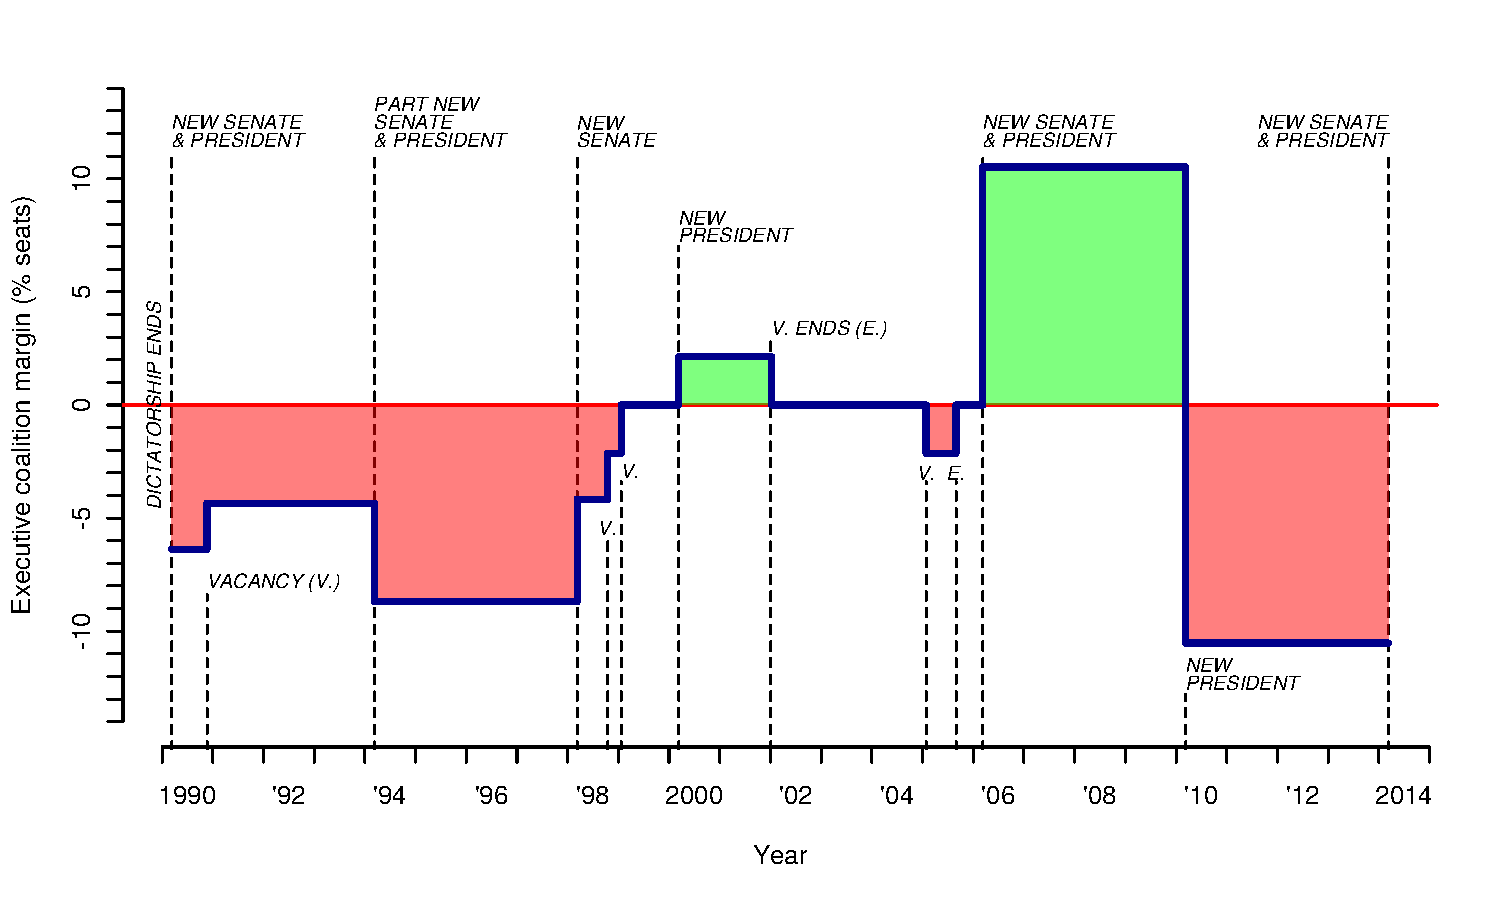
\includegraphics[width=\columnwidth]{../graphs/senChile.pdf}
  \caption{The Conservative chamber. The blue, crenellated line reports, longitudinally, the percentage of Senate seats controlled by the president's coalition minus the percentage controlled by the opposition. Totals include 38 elected senators and, up to 2006, 9 appointed senators and two or fewer senators for life. Vacancies, if any, are excluded; see text for details. The Senate renews in full every eight years, and was partially renewed in 1994. Vacancies reported: Ruiz Danyau, Air Force appointee, died in office 11/1990; Pinochet detained in London 10/1998; Errázuriz stripped of immunity 1/1999 (resinstated 1/2002); Lavandero stripped of immunity 1/2005 (replaced upon conviction 8/2005). }\label{f:senChile}
\end{center}
\end{figure}

\section{Bicameral rules}

Chilean bicameralism operates on a limited navette and conference sequence \citep{tsebelis.money.1997,londregan.2000a}. Bills can originate in the chamber of deputies or the senate, by motion of any member to the parent chamber or by message from the executive. They need approval in both chambers of Congress, but the rules to approve can vary drastically. Bicameral negotiation begins with a single trip of a French-style navette: bills are considered and voted in the origin chamber first; if approved, they migrate to the revising chamber for consideration and vote. If it concurs, the bill is sent to the executive for signature. But if the revising chamber rejects, or the origin chamber finds amendments to the bill unacceptable, the chambers appoint five members each to a U.S.-style conference committee to agree on a compromise that each chamber must subsequently vote up or down. 

\begin{figure}
  \begin{center}
  \begin{tabular}{cc}
    (a) bill rejected by $c_1$ & (b) $c_1$ rejects bill amended by $c_2$ \\
    \tikzstyle{mid}=[circle,draw]
    \begin{tikzpicture}
      \node[mid] at (2,0) (l) {\emph{e}}; 
      \node[mid] at (4,1) (e) {\emph{$c_2$}}; 
      \node[mid] at (6,0) (v) {\emph{$c_1$}}; 
      \node at (4,-1) (le) {$x_0$}; 
      \node at (6,2) (ee) {$x_0$}; 
      \node at (8,1) (ve1) {$x_0$}; 
      \node at (8,-1) (ve2) {$x$};
      \path[-] (l) edge node [above, sloped] {\footnotesize{insist}} (e) (e) edge node [below, sloped] {\footnotesize{$aye\geq\frac{2}{3}$}} (v);
      \path[-o] (l) edge node [below, sloped] {\footnotesize{no}} (le) (e) edge node [above, sloped] {\footnotesize{$nay>\frac{1}{3}$}} (ee) (v) edge node [above, sloped] {\footnotesize{$nay>\frac{2}{3}$}} (ve1) edge node [below, sloped] {\footnotesize{$aye\geq\frac{1}{3}$}} (ve2);
    \end{tikzpicture} 
    &
    \tikzstyle{mid}=[circle,draw]
    \begin{tikzpicture}
      \node[mid] at (2,0) (l) {\emph{e}}; 
      \node[mid] at (4,1) (e) {\emph{$c_1$}}; 
      \node[mid] at (6,0) (v) {\emph{$c_2$}}; 
      \node at (4,-1) (le) {$x_0$}; 
      \node at (6,2) (ee) {$x_0$}; 
      \node at (8,1) (ve1) {$x_0$}; 
      \node at (8,-1) (ve2) {$x$};
      \path[-] (l) edge node [above, sloped] {\footnotesize{insist}} (e) (e) edge node [below, sloped] {\footnotesize{$aye>\frac{1}{3}$}} (v);
      \path[-o] (l) edge node [below, sloped] {\footnotesize{no}} (le) (e) edge node [above, sloped] {\footnotesize{$nay\geq\frac{2}{3}$}} (ee) (v) edge node [above, sloped] {\footnotesize{$nay>\frac{1}{3}$}} (ve1) edge node [below, sloped] {\footnotesize{$aye\geq\frac{2}{3}$}} (ve2);
    \end{tikzpicture} 
    \\
    \end{tabular}
  \caption{Two second chance (\emph{insistencia}) sequences. Nodes indicate moves by $e=$ executive, $c_1=$ chamber rejecting the bill, and $c_2=$ other cchamber.}\label{f:swapException}
  \end{center}
\end{figure}

Exceptions apply, leading to bicameral rules variation. There is a general restrictive rule, which the president can invoke in most circumstances, granting rejected bills a second chance.\footnote{The sole circumstance when a rejected bill cannot be given a second chance ensues when, following rejection by the revising chamber, a compromise is reached in conference, accepted in the origin chamber, but rejected by the revising. See Const.\ art.\ 70, and compare to 68 and 71.} When the procedure known as \emph{insistencia} is invoked, rejection of the bill by the recalcitrant chamber requires a two-thirds of members present vote. Passage by the other chamber also becomes more difficult, demanding a two-thirds of members present favorable vote. Figure \ref{f:swapException} illustrates the sequence of the second chance rule the asymmetry introduced for proponents and opponents alike. Two variants are considered, one applicable to executive-initiated bills rejected in the origin chamber or bills rejected in the revising chamber (part a); the other applicable to bills amended in the revising chamber that are rejected in the origin chamber (parb b). 

\begin{figure}
  \begin{center}
    \tikzstyle{mid}=[circle,draw]
    \begin{tikzpicture}
      \node[mid] at (-2,0) (A) {$A$}; 
      \node[mid] at (0,1) (N) {$N$}; 
      \node[mid] at (2,0) (e) {$e$}; 
      \node[mid] at (4,1) (a) {$a$}; 
      \node[mid] at (6,0) (n) {$n$}; 
      \node at (0,-1) (Ae) {$x_0$}; 
      \node at (2,2) (Ne) {$x$}; 
      \node at (4,-1) (ee) {$x_0$}; 
      \node at (6,2) (ae) {$x_0$}; 
      \node at (8,1) (ne1) {$x_0$}; 
      \node at (8,-1) (ne2) {$x$};
      \path[-] (e) edge node [above, sloped] {\footnotesize{insist}} (a) (a) edge node [below, sloped] {\footnotesize{aye}} (n);
      \path[-o] (e) edge node [below, sloped] {\footnotesize{no}} (ee) (a) edge node [above, sloped] {\footnotesize{nay}} (ae) (n) edge node [above, sloped] {\footnotesize{nay}} (ne1) edge node [below, sloped] {\footnotesize{aye}} (ne2);
      \path[-] (A) edge node [above, sloped] {\footnotesize{pro-}} (N) (A) edge node [below, sloped] {\footnotesize{pose $x$}} (N) (N) edge node [below, sloped] {\footnotesize{reject}} (e);;
      \path[-o] (A) edge node [below, sloped] {\footnotesize{no}} (Ae) (N) edge node [above, sloped] {\footnotesize{accept}} (Ne);
    \end{tikzpicture} 
  \caption{The second chance game (\emph{insistencia}). Nodes indicate moves by $A,N=$ majorities in each chamber, $e=$ executive, $n=$ pivotal rejection member, and $a=$ pivotal approval member.}\label{f:2chanceGame}
  \end{center}
\end{figure}

Figure \ref{f:2chanceGame} stylizes the restrictive rule as a game between the executive ($e$) and members of both chambers of Congress. $N$ and $A$ command majorities in the chamber that rejected a bill (the nay chamber) and the chamber where it gets a second chance (the aye chamber), respectively; $n$ is the last member needed for two-thirds coalition against in the nay chamber, $a$ the last member needed for a two-thirds coalition for the bill in the aye chamber. $A$ makes a proposal that $N$ may accept or reject. If the latter, the executive may opt to insist, letting $a$ end the game or give $n$ a chance to slect between the proposal and the status quo. If played with full information, the sequence reveals that $N$'s limit to oppose a bill pleasing a supermajority of the other chamber and the executive depends on $n$'s (one third of the nay chamber) preferences. 

This is important because of incongruence between the senate and chamber. Say how...

The restrictive rule should interact with urgencies. Consider the casae where the recalcitrant chamber will accept only if its amendments hold. Doing so, may prompt a second chance and they could lose. Rejecting may achieve the same. In such circumstances, the optimal choice would be not to act on the bill. But the president can force them to do so. 

% see Dec. 2014 notebook, p. 2 for picture of one equilibrium path for the game
\begin{figure}
  \begin{center}
    \begin{tikzpicture}
      \draw (0,0) -- (10,0);
    \end{tikzpicture} 
  \caption{Bicameral negotiation with second chance rule}\label{f:2chanceEql}
  \end{center}
\end{figure}

\section{Descriptives}

About seven thousand bills were introduced to Congress between 1998 and 2014, 438 yearly on average. Unlike the U.S., the executive can initiate legislation directly. The president introduced one bill for every four by members of Congress, with markedly different success rates. Less than one in ten legislative bill passed, while more than seven in ten executive bills did so. Overall, legislators authored about one law for every three by the president (see Table \ref{T:billDescriptives}).

\begin{table}
\begin{center}
\begin{tabular}{lrrr}
                         &  by           &  by          &    by      \\
Bills                    &  legislators  &  president   &    ~~~~either  \\ \hline
introduced               &         5533  &        1469  &      7002  \\
as \%                    &    \emph{79}  &   \emph{21}  & \emph{100} \\ \hdashline
passed                   &          404  &        1066  &      1470  \\
as \%                    &    \emph{27}  &   \emph{73}  & \emph{100} \\
as \% introduced         &     \emph{7}  &   \emph{73}  &  \emph{21} \\ \hdashline
with urgency message(s)  &          351  &        1016  &      1367  \\
as \%                    &    \emph{26}  &   \emph{74}  & \emph{100} \\
as \% introduced         &     \emph{6}  &   \emph{69}  &  \emph{20} \\
as \% passed             &    \emph{87}  &   \emph{95}  &  \emph{93} \\ \hline
\end{tabular}
\caption{Bills, laws, and urgency messages 1998--2014}\label{T:billDescriptives}
\end{center}
\end{table}


% \begin{tabular}{lrrrrrr}
%                                   &  \mc{2}{c}{passed}    &  \mc{2}{c}{not}     &  \mc{2}{c}{all}      \\    
% Bills with urgency in             &  N     &  \%          &  N     &  \%        &  N     &  \%         \\ \hline
% $1^{st}$ chamber only              &   122  &  \emph{32}   &   259  &  \emph{68} &   381  &  \emph{100} \\
% $2^{nd}$ chamber only              &   129  &  \emph{68}   &    62  &  \emph{32} &   191  &  \emph{100} \\
% conference only                   &    27  &  \emph{82}   &     6  &  \emph{18} &    33  &  \emph{100} \\
% $1^{st}$ and $2^{nd}$               &   363  &  \emph{81}   &    87  &  \emph{19} &   450  &  \emph{100} \\
% $1^{st}$ and conference            &    39  &  \emph{93}   &     3  &  \emph{7}  &    42  &  \emph{100} \\
% $2^{nd}$ and conference            &    37  &  \emph{90}   &     4  &  \emph{10} &    41  &  \emph{100} \\
% $1^{st}$, $2^{nd}$, and conference  &   212  &  \emph{94}   &    14  &  \emph{6}  &   226  &  \emph{100} \\
% no urgency                        &   541  &  \emph{10}   &  5097  &  \emph{90} &   5638 &  \emph{100} \\ \hline
% %total                             &   929  &  \emph{68}   &   435  &  \emph{32} &  1364  &  \emph{100} \\ \hline
% \end{tabular}

An urgency message can be sent at any stage of the bicameral legislative process, compelling the chamber receiving it to act on a bill. Since urgencies expire once the chamber has finished, it is not uncommon for presidents to send messages at more than one step. Two-fifths of bills with urgencies were deemed so in two or three steps of the legislative process---the first chamber, the second, and/or the bicameral conference.    

\begin{table}
\begin{center}
\begin{tabular}{lrrr|rrr}
                                  &  \mc{6}{c}{Proposer}                                               \\    
                                  &  \mc{3}{c}{president}         &  \mc{3}{c}{member of Congress}             \\    
Bills with urgency in             &  \% pass   & \% not    & ~~~~~N &  \% pass  & \% not    & ~~~~~N \\ \hline
$1^{st}$ chamber only              &  \emph{40} & \emph{60} & 278  & \emph{12} & \emph{88} & 103  \\
$2^{nd}$ chamber only              &  \emph{84} & \emph{16} &  98  & \emph{51} & \emph{49} &  93  \\
conference only                   &  \emph{95} & \emph{5}  &  20  & \emph{62} & \emph{38} &  13  \\
$1^{st}$ and $2^{nd}$               &  \emph{86} & \emph{14} & 369  & \emph{58} & \emph{42} &  81  \\
$1^{st}$ and conference            &  \emph{92} & \emph{8}  &  39  & \emph{100}& \emph{0}  &   3  \\
$2^{nd}$ and conference            &  \emph{100}& \emph{0}  &  18  & \emph{83} & \emph{17} &  23  \\
$1^{st}$, $2^{nd}$, and conference  &  \emph{94} & \emph{6}  & 192  & \emph{91} & \emph{9}  &  34  \\
no urgency                        &  \emph{67} & \emph{33} & 455  & \emph{5}  & \emph{95} & 5183  \\ \hline
\end{tabular}
\caption{The legislative process, urgency messages, and bill passage by proposer 1998--2014}\label{T:stepsUrgencyPass}
\end{center}
\end{table}

\begin{table}
\begin{center}
\begin{tabular}{rrr}
Number of &      Bill &     \\
messages  & frequency &  ~~~~~~~~\% \\ \hline
%None              &  5635     &     \\
1                 &  215      &  \emph{15}   \\
2                 &  244      &  \emph{17}   \\
3                 &  145      &  \emph{10}   \\
4                 &  115      &  \emph{8}    \\
5                 &  104      &  \emph{7}    \\
6-10              &  236      &  \emph{16}   \\
11-20             &  185      &  \emph{13}   \\
21-40             &  99       &  \emph{7}    \\
41-71             &  123      &  \emph{8}    \\
Total             & 1466      & \emph{100}   \\ \hline
\end{tabular}
\caption{Urgent bills classified by number of urgency messages received}\label{T:billFreqByNurg}
\end{center}
\end{table}

\begin{table}
\begin{center}
\begin{small}
\begin{tabular}{lrrrrrrrr}
                         &  \mc{8}{c}{Percent Concertación sponsors} \\
Urgency raised by        &  0\%      &  1--25\%  &  26--50\%  &  51--75\%  &  76--99\%  &  100\%      &  All         &  N \\ \hline
Concertación presidents  & \emph{21} & \emph{3}  & \emph{10}  & \emph{15}  & \emph{13}  & \emph{39}   &  \emph{100}  &  230 \\
Right president          & \emph{26} & \emph{4}  & \emph{18}  & \emph{12}  & \emph{12}  & \emph{26}   &  \emph{100}  &  121 \\
\end{tabular}
\caption{Sponsorship of MC-initiated bills receiving at least one urgency messages. Entries are relative frequencies of Concertación sponsors among bills declared urgent by presidents elected by a given list. The first entry reports that 21 percent of bills declared urgent by a Concertación president had not a single sponsor elected by that list; and so forth.}\label{T:sponsorsOfUrgBills}
\end{small}
\end{center}
\end{table}



\section{Dependent variable}

The abundance of urgency messages is remarkable. Not taking the February Summer break into account,\footnote{Three February weeks with urgency messages are retained in the count.} when Congress rarely convenes, less than one in three weeks in the period were free of urgency messages. The executive sent 7.6 weekly messages on average to the chamber of deputies, and 10.5 to the senate.

%   Cámara  
% ##########
%    Min. 1st Qu.  Median    Mean 3rd Qu.    Max. 
%   0.000   0.000   4.000   7.602  11.000  85.000 
%   Senado  
% ##########
%    Min. 1st Qu.  Median    Mean 3rd Qu.    Max. 
%    0.00    0.00    5.00   10.49   14.00   97.00 


\begin{figure}
\begin{center}
\begin{tabular}{cccc}
    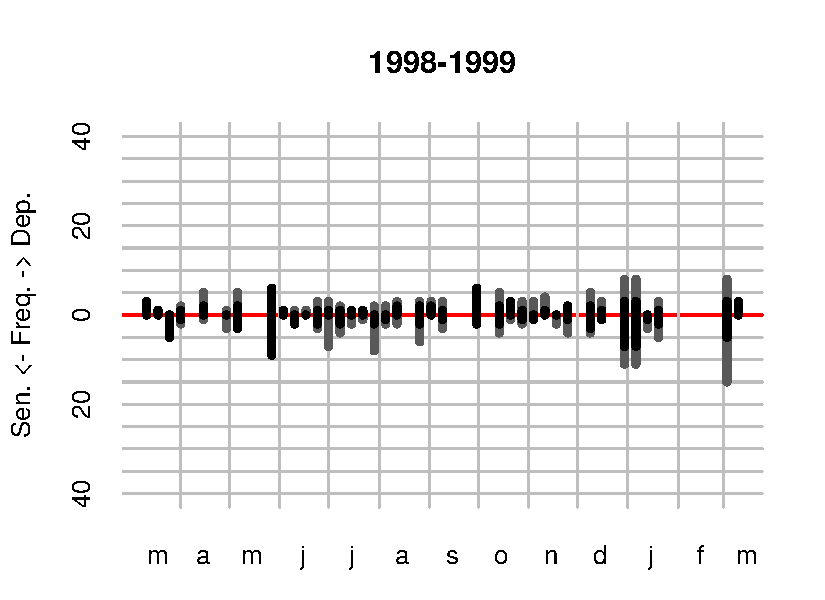
\includegraphics[width=.22\columnwidth]{../graphs/urgenciasHistog1998.pdf} &
    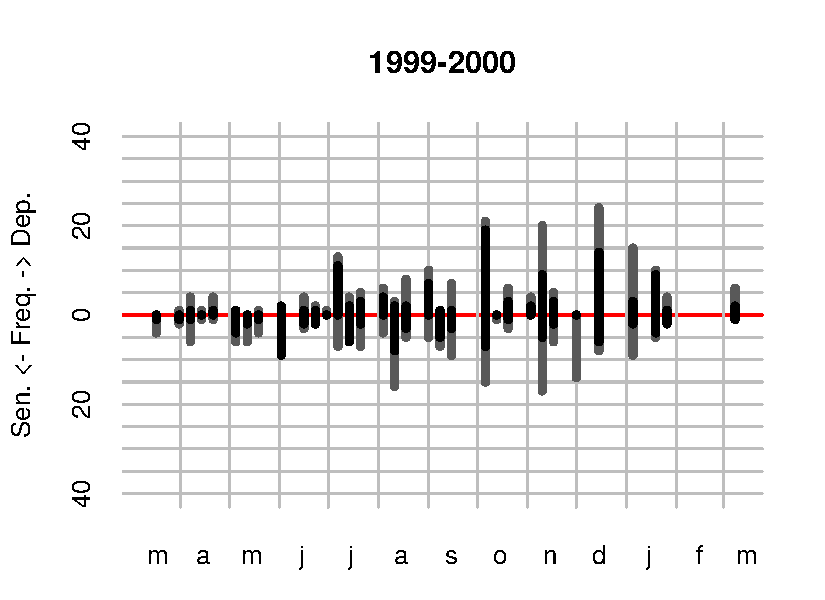
\includegraphics[width=.22\columnwidth]{../graphs/urgenciasHistog1999.pdf} &
    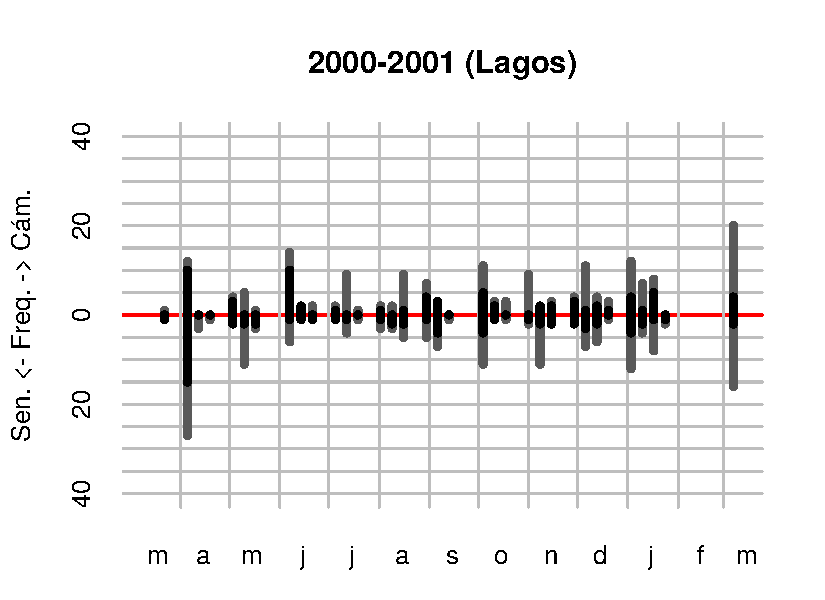
\includegraphics[width=.22\columnwidth]{../graphs/urgenciasHistog2000.pdf} &
    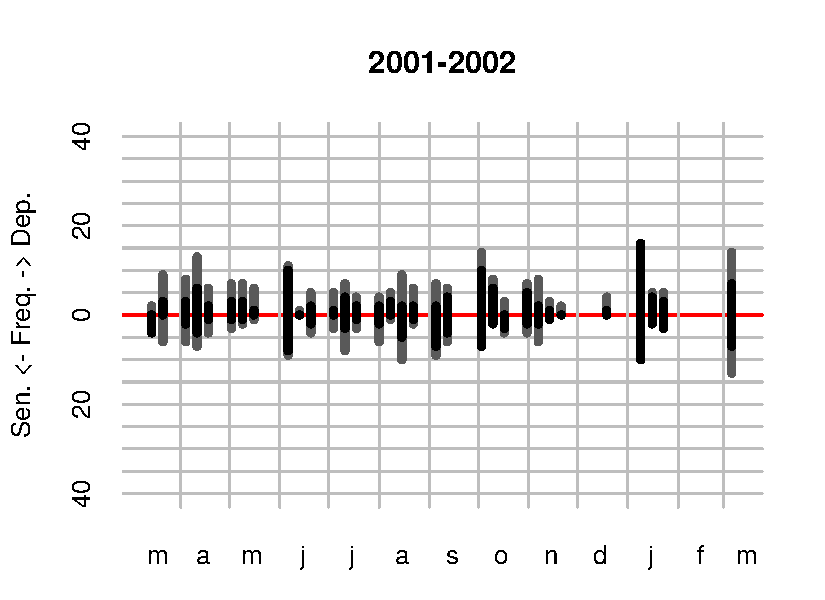
\includegraphics[width=.22\columnwidth]{../graphs/urgenciasHistog2001.pdf} \\
    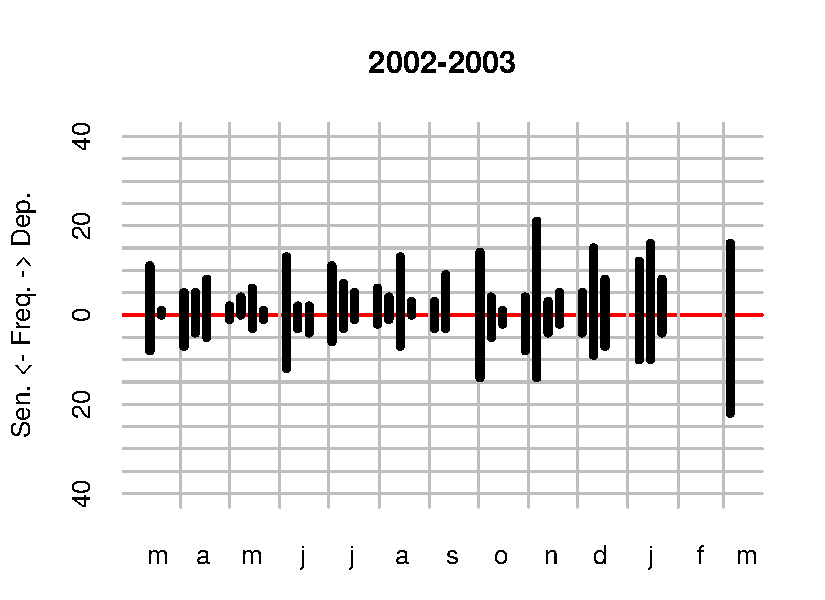
\includegraphics[width=.22\columnwidth]{../graphs/urgenciasHistog2002.pdf} &
    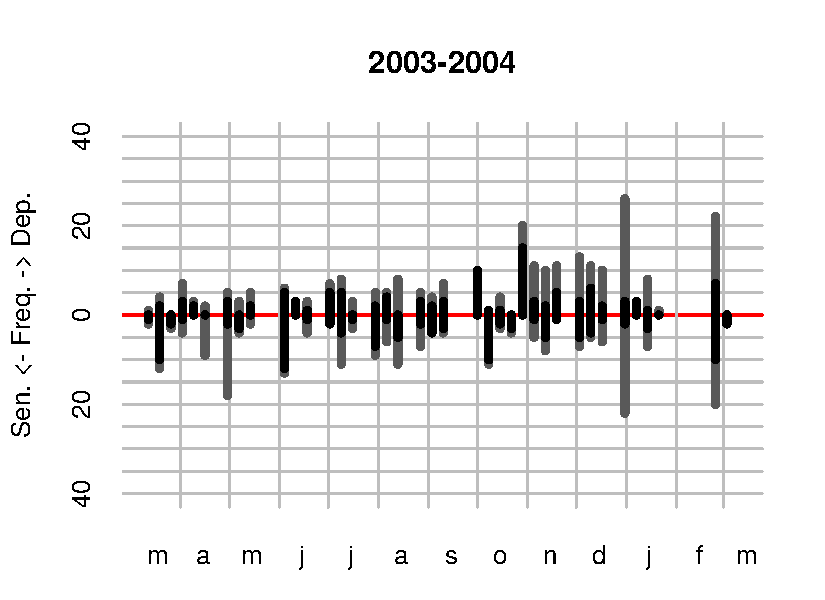
\includegraphics[width=.22\columnwidth]{../graphs/urgenciasHistog2003.pdf} &
    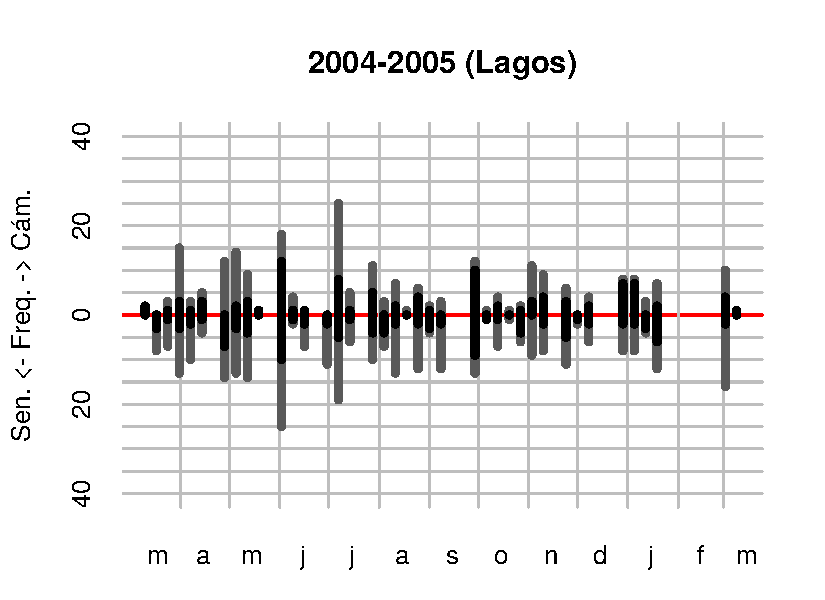
\includegraphics[width=.22\columnwidth]{../graphs/urgenciasHistog2004.pdf} &
    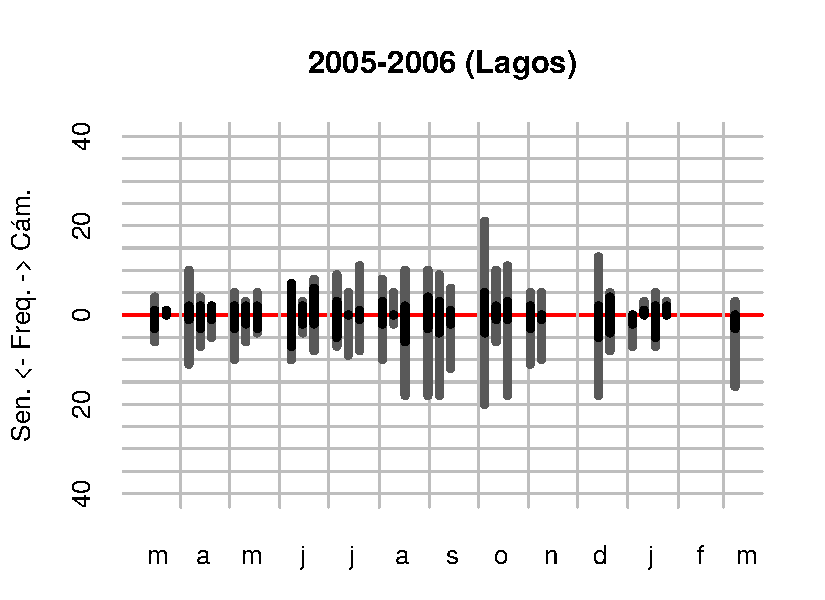
\includegraphics[width=.22\columnwidth]{../graphs/urgenciasHistog2005.pdf} \\
    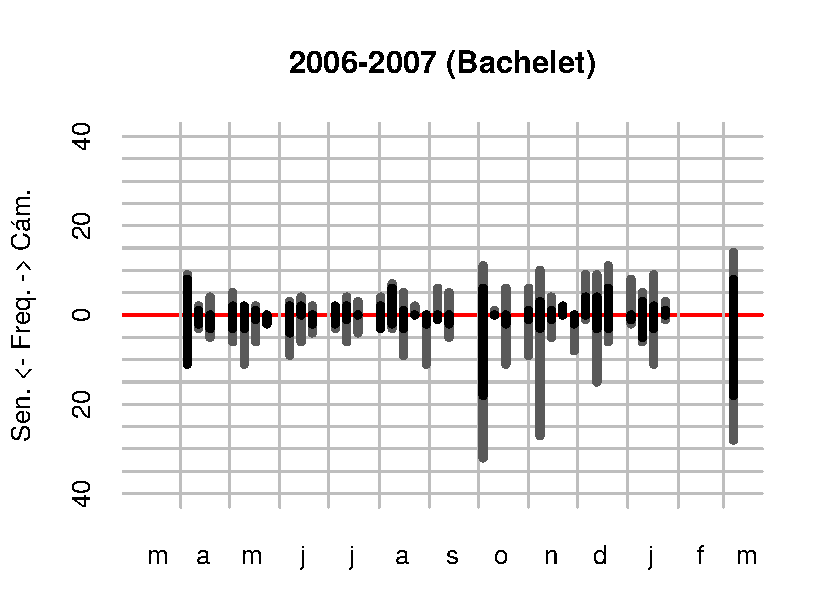
\includegraphics[width=.22\columnwidth]{../graphs/urgenciasHistog2006.pdf} &
    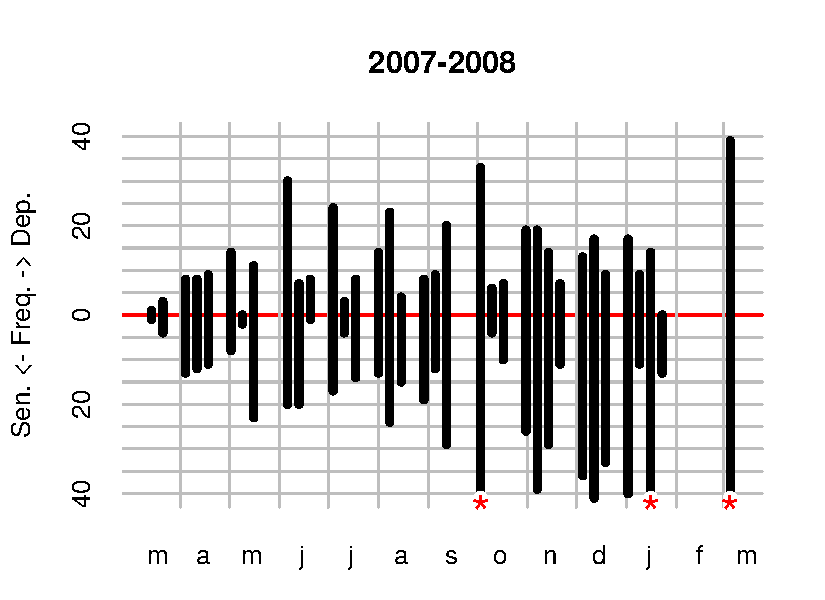
\includegraphics[width=.22\columnwidth]{../graphs/urgenciasHistog2007.pdf} &
    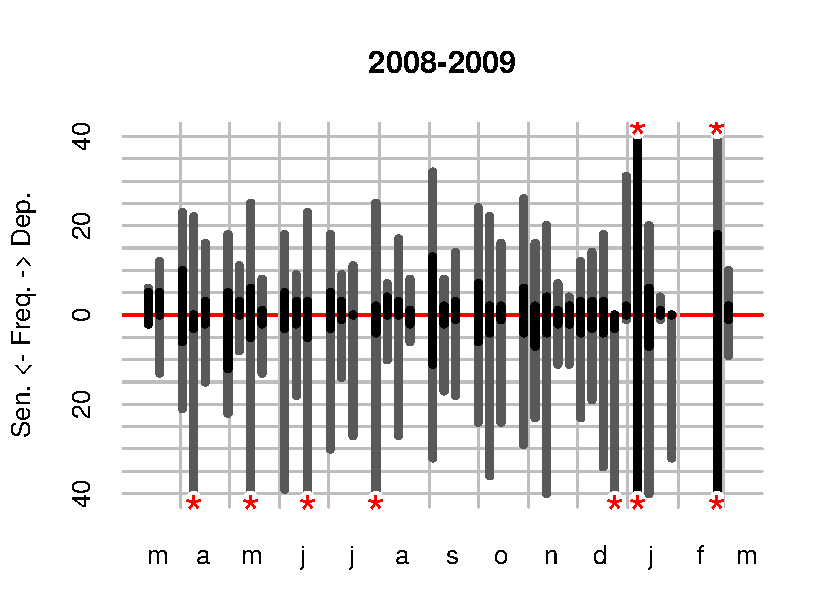
\includegraphics[width=.22\columnwidth]{../graphs/urgenciasHistog2008.pdf} &
    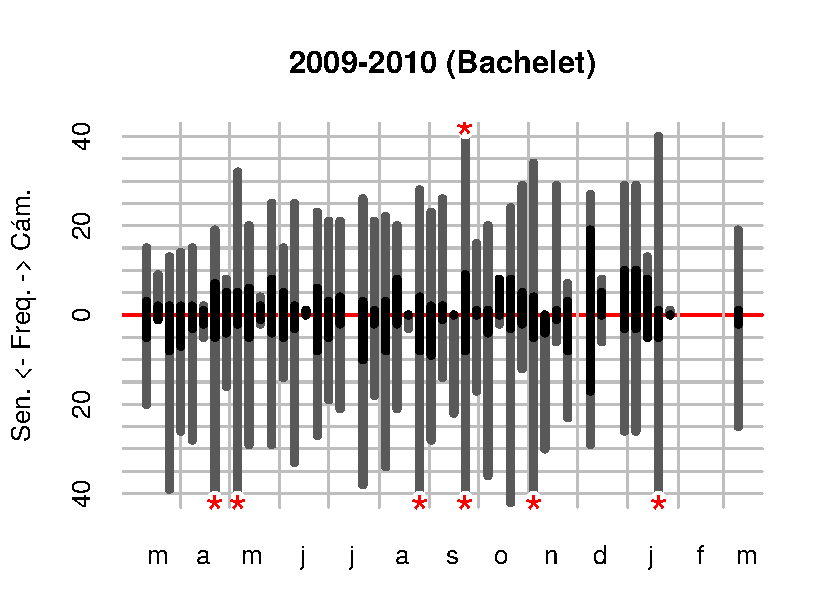
\includegraphics[width=.22\columnwidth]{../graphs/urgenciasHistog2009.pdf} \\
    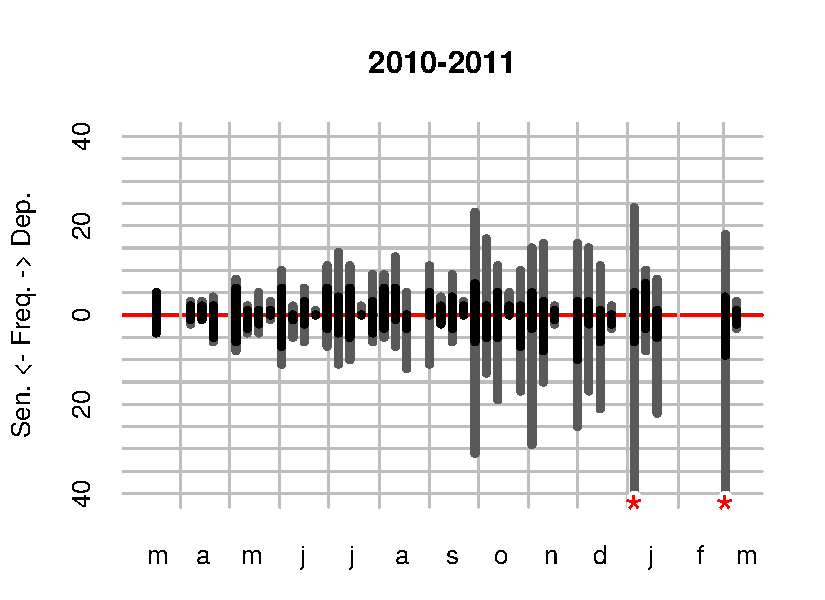
\includegraphics[width=.22\columnwidth]{../graphs/urgenciasHistog2010.pdf} &
    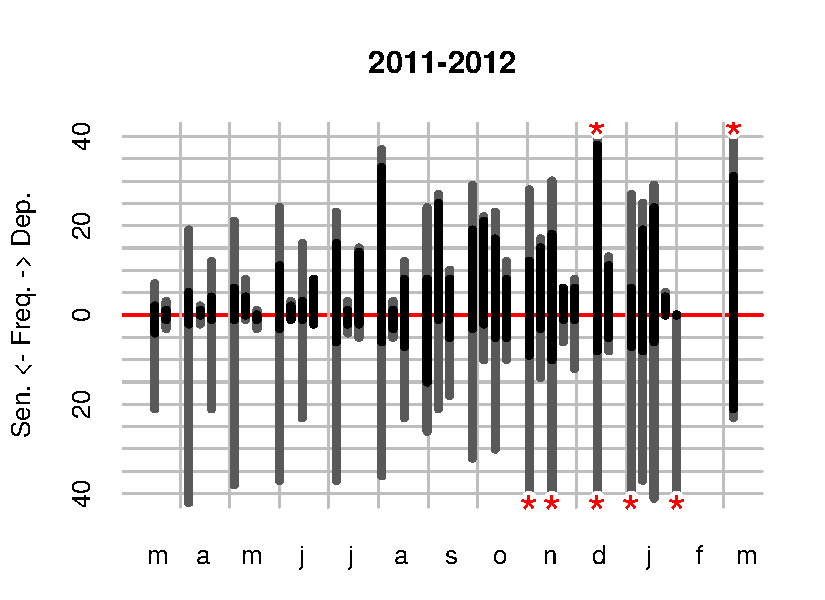
\includegraphics[width=.22\columnwidth]{../graphs/urgenciasHistog2011.pdf} &
    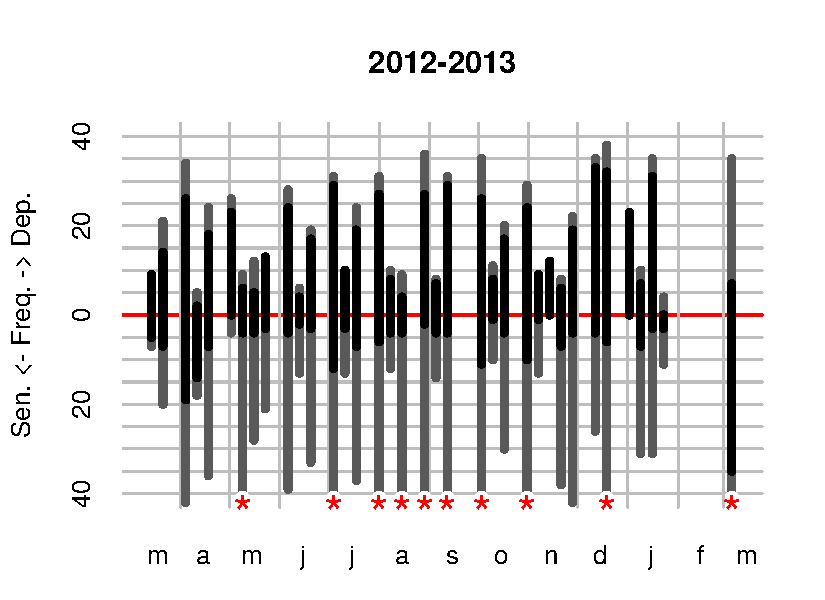
\includegraphics[width=.22\columnwidth]{../graphs/urgenciasHistog2012.pdf} &
    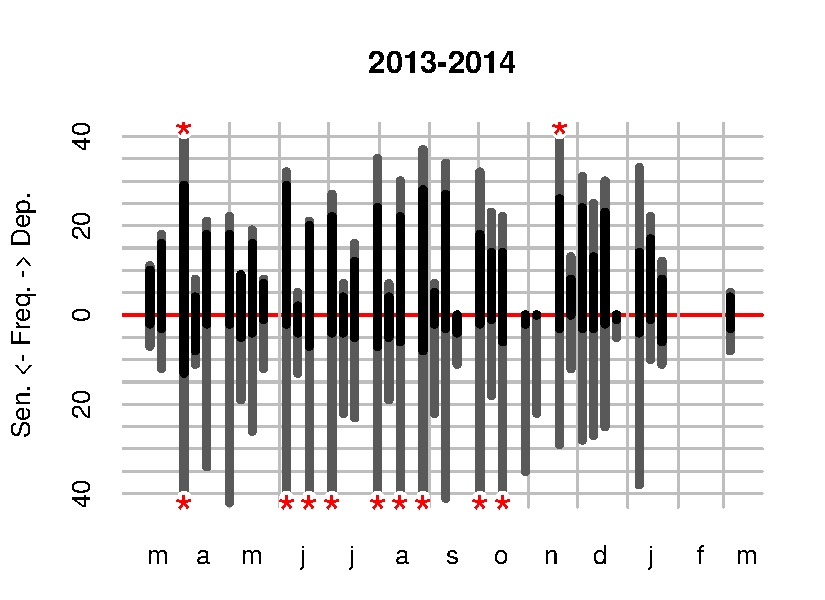
\includegraphics[width=.22\columnwidth]{../graphs/urgenciasHistog2013.pdf} \\
\end{tabular}
  \caption{Weekly urgencies by legislative year. Deputies histogram above, Senate below the zero line. Asterisk atop column indicates off-the-chart urgency message frequency. Source: prepared with data from the Chilean Congress.}\label{f:depvarHistog}
\end{center}
\end{figure}


There are detailed plots, keep only one year

% \begin{sidewaysfigure}
% \begin{center}
%     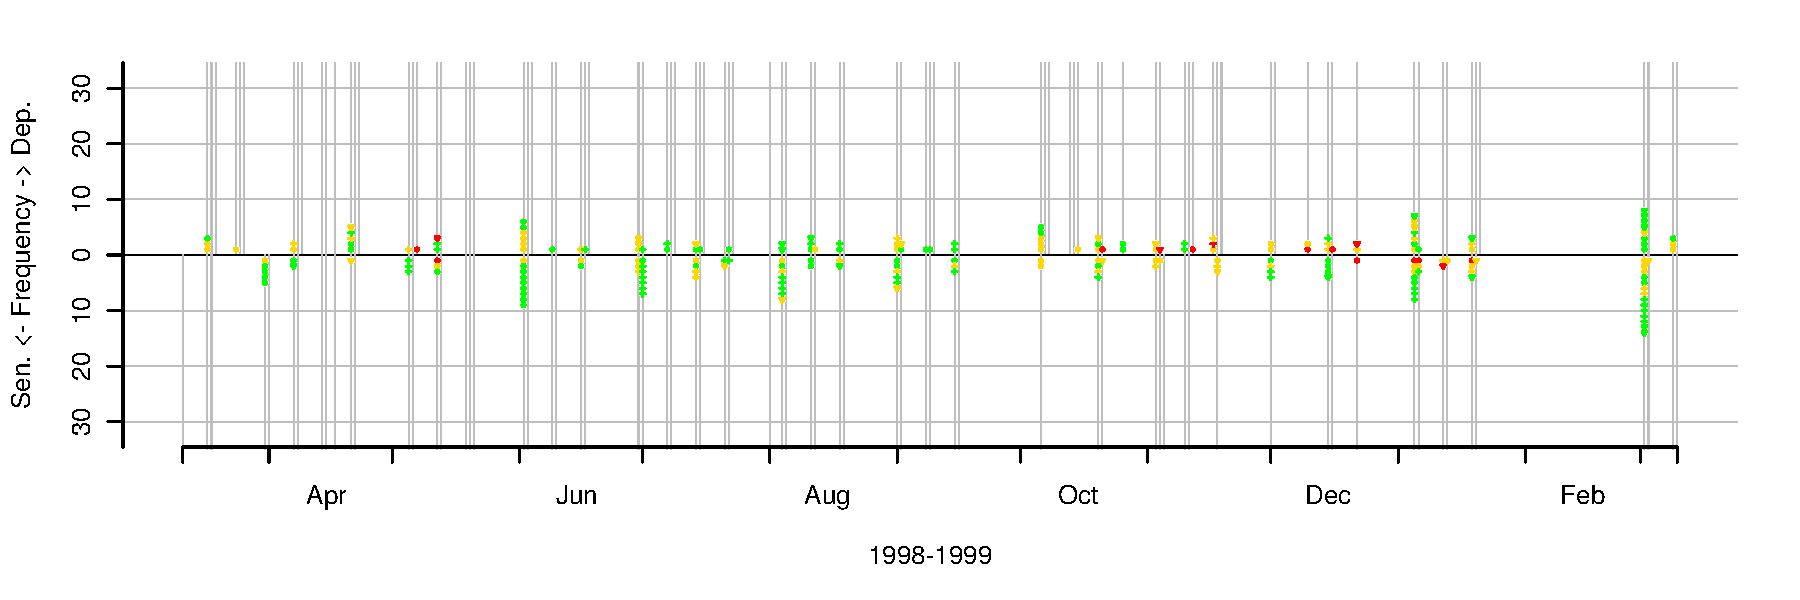
\includegraphics[width=\columnwidth]{../graphs/urgencias1998.pdf} \\
%     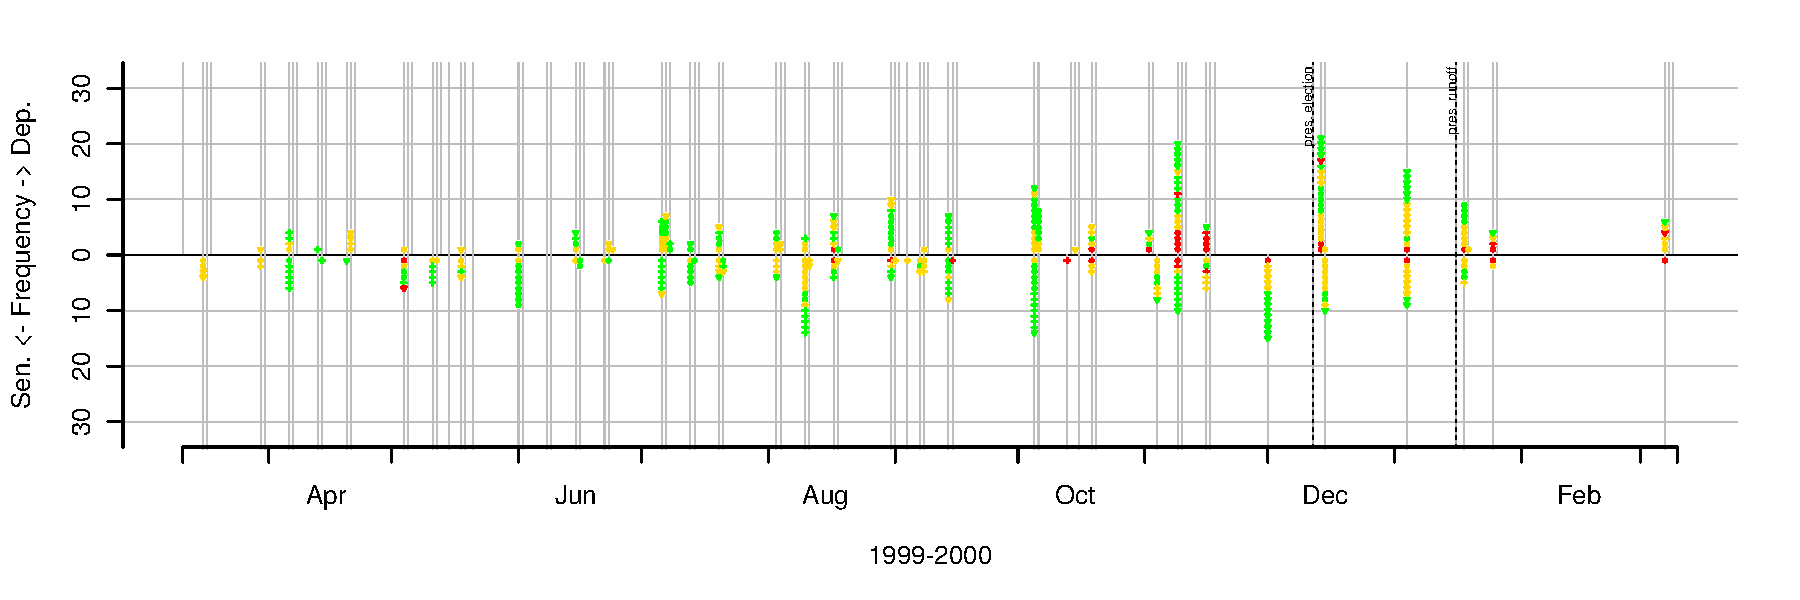
\includegraphics[width=\columnwidth]{../graphs/urgencias1999.pdf} 
%   \caption{Urgencies by legislative year. Deputies and Senate histograms above and below the zero line, respectively. Vertical grey lines indicate that a session took place. One point for each urgency message, a circle for a newly declared urgent bill, a plus sign for an urgent bill with new deadline, an inverted triangle for a retired urgency. Point color indicates the urgency deadline, red for 3/6 days, yellow for 10/15 days, green for 30 days. Parentheses atop columns indicate off-the-chart urgency message frequency.}\label{f:depvar}
% \end{center}
% \end{sidewaysfigure}

% \begin{sidewaysfigure}\ContinuedFloat
% \begin{center}
%     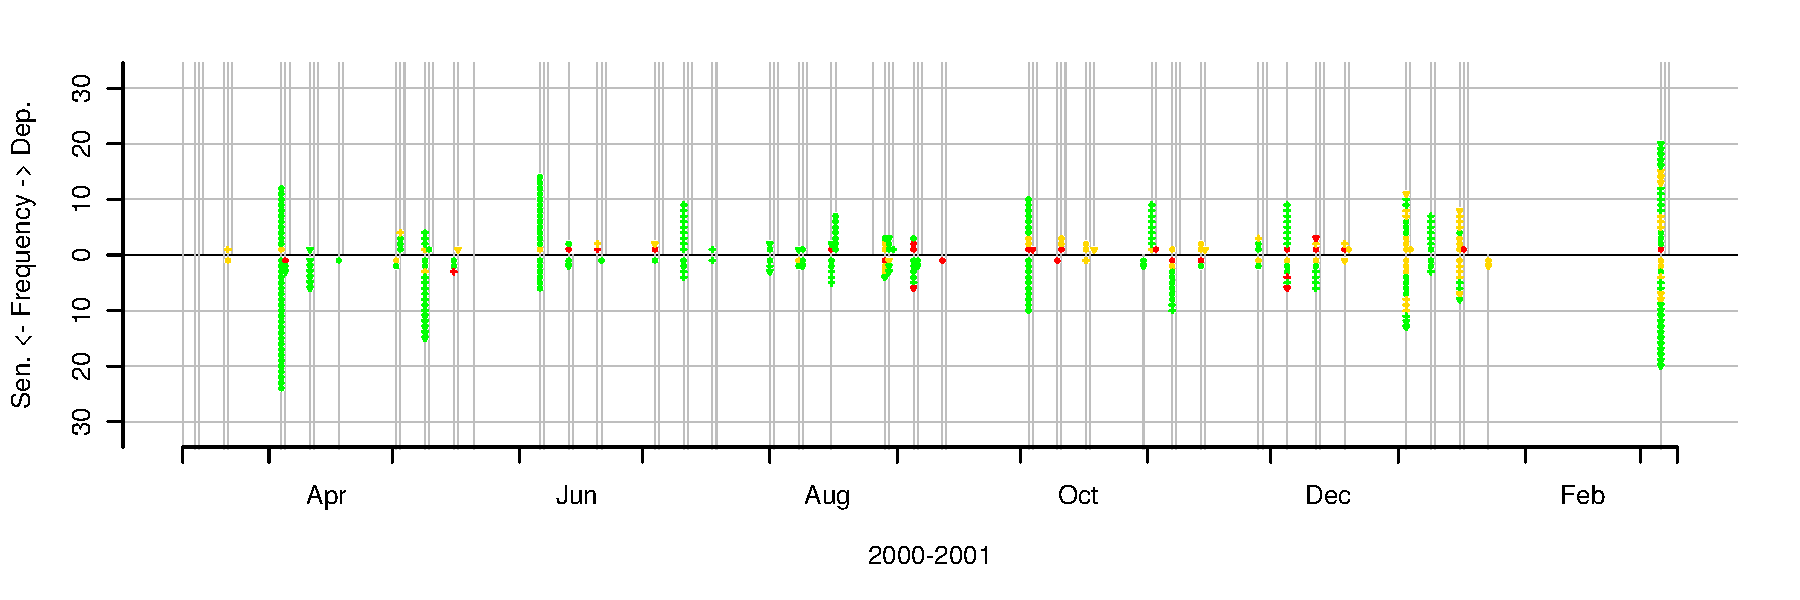
\includegraphics[width=\columnwidth]{../graphs/urgencias2000.pdf} \\
%     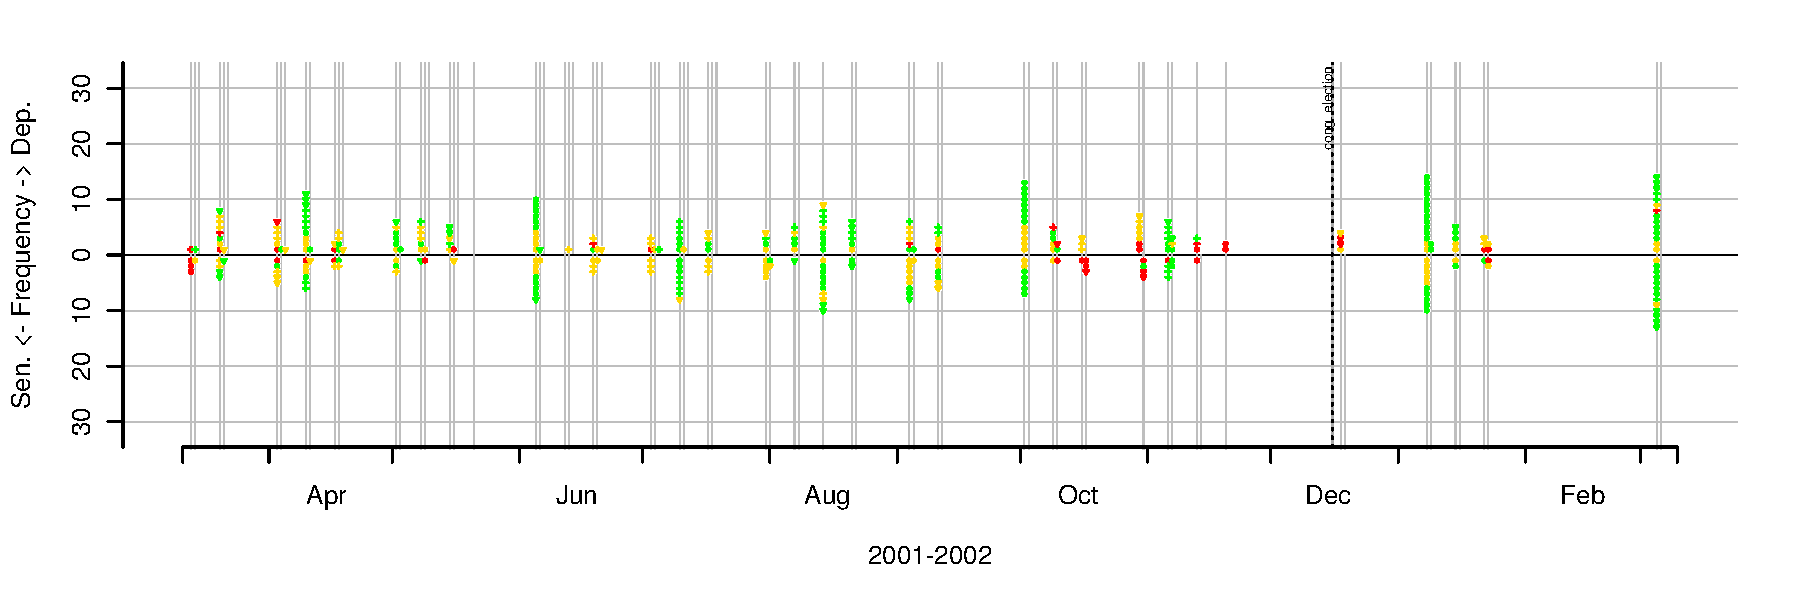
\includegraphics[width=\columnwidth]{../graphs/urgencias2001.pdf} 
%   \caption{Urgencies by legislative year (cont.)}\label{f:depvar}
% \end{center}
% \end{sidewaysfigure}

\begin{figure}
\begin{center}
    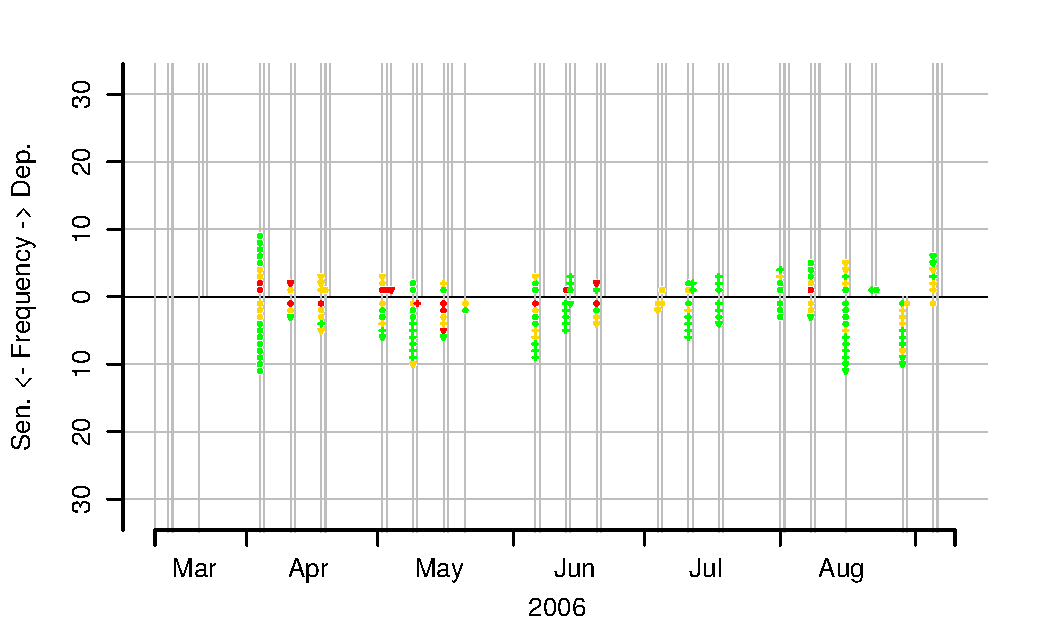
\includegraphics[width=\columnwidth]{../graphs/urgencias2006-1.pdf} \\
    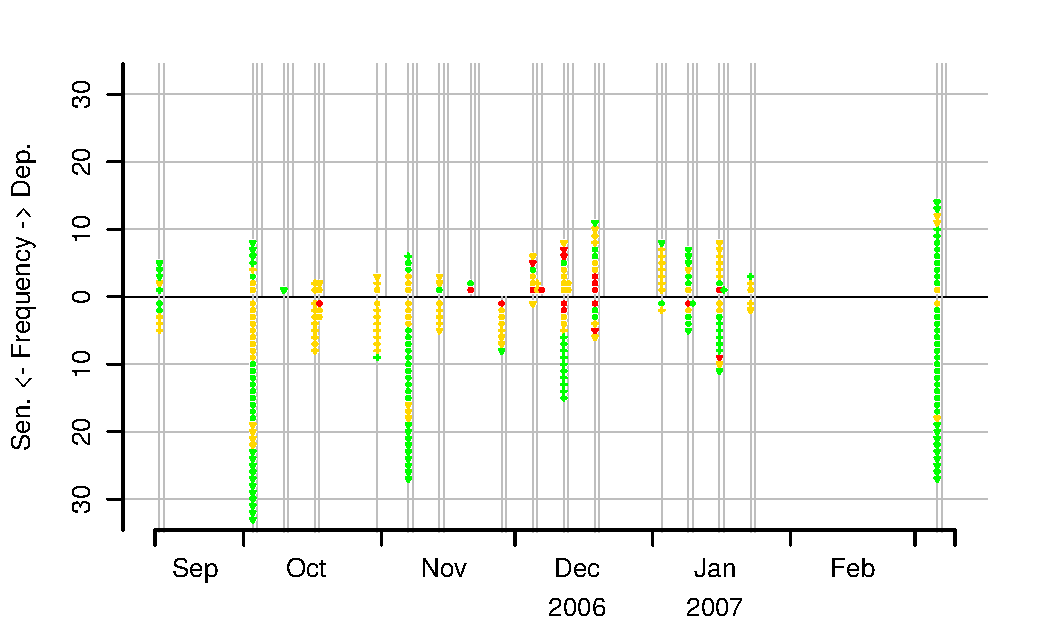
\includegraphics[width=\columnwidth]{../graphs/urgencias2006-2.pdf} 
  \caption{Urgencies in one legislative year. Deputies and Senate data above and below the zero line, respectively. Vertical grey lines indicate that a session took place. One point for each urgency message, a circle for a newly declared urgent bill, a plus sign for an urgent bill with new deadline, an inverted triangle for a retired urgency. Point color indicates the urgency deadline, red for 3/6 days, yellow for 10/15 days, green for 30 days. Parentheses atop columns indicate off-the-chart urgency message frequency.}\label{f:depvar}
\end{center}
\end{figure}

\section{extras}

\section{In the law}

Formal authority to interfere in the Congressional agenda is established in the Constitution (art.\ 74) and Congressional Organic Law (arts.\ 26 and 27). The constitution stipulates that the president can urge action on any bill at any stage in the legislative process. The chamber receiving the urgency message is compelled to act on the bill (``discuss and vote it'') before a specific deadline. Since inter-cameral differences are dealt with in conference (\emph{comisión mixta}, const.\ arts.\ 68--70), an urgency message at this stage compells Congress (ie.\ the conference and both chambers) to act before the deadline. The law defines the breadth of the interference, giving the president a choice of 30-day (simple urgency), 10-day (extreme urgency), or 3-day (immediate discussion) deadlines. As of July 2010, when the constitution was amended, the deadlines for the extreme and immediate urgencies were relaxed to 15 and 6 days, repsectively. So at its maximum---an immediate discussion urgency to a bill in conference before 2010---the conference has one business day to report a compromise bill, and each chamber one day each to push the bill to the floor and vote it up or down.\footnote{Congressional practice is well summarized by the library of Congress at \url{http://www.bcn.cl/ecivica/formacion/}.} The president can retire the urgency at will, with immediate effects. Urgencies expire at the end of the regular session. 

Urgent bills take precedence in the day's order, the . How exactly? It affects one of 30/15/6 successive days. 

How is the day's order prepared? ``Las urgencias determinan el orden de la tabla de discusión'')

What if Congress fails to act? Can urgency be ignored? Can a committee report kill the bill or does urgency compell a vote in the floor (law's art.\ 27 ``su discusión y votación en la Cámara requerida deberán quedar terminadas en el plazo'')?

\section{Data}

The Chamber of Deputies' web page (\url{www.camara.cl}) has detailed information on bill histories, including business in the Senate, since the return to democracy in 1990. A request of information was sent by email to the Congressional staff. Upon their failure to respond, site contents were scraped. The javascript-rich web page posed difficulties for this, resolved with \texttt{Python}'s \texttt{Selenium} library. The script (posted in a web appendix at...) was inefficient (slow) but effectively downloaded bill histories for seven legislatures between March 1, 1990 and February 28, 2014. 

\begin{table}
\begin{center}
\begin{tabular}{rrrrrrrrrrr}
       & \mc{10}{c}{$N$ (and \%) bills reporting urgency} \\ \cline{2-11}
       & \mc{2}{c}{in messages}  & \mc{2}{c}{in timeline} &      &                  & &                     & & \\          
       & \mc{2}{c}{but not}      & \mc{2}{c}{but not}     & \mc{2}{c}{in both}      & &                     & \mc{2}{c}{All} \\
Period & \mc{2}{c}{in timeline}  & \mc{2}{c}{in messages} & \mc{2}{c}{tabs}         & \mc{2}{c}{in neither} & \mc{2}{c}{bills} \\ \hline
%           ~UH                     U~H                       UH                        ~U~H             
1990--1994  &  213  &   \emph{(19)}  &   5  &  \emph{(.4)}  &    25   &   \emph{(2)}  &   897  &  \emph{(79)}  &  1,140  &  \emph{(100)} \\
1994--1998  &  168  &   \emph{(17)}  &      &               &    18   &   \emph{(2)}  &   775  &  \emph{(81)}  &    961  &  \emph{(100)} \\
1998--2002  &  128  &   \emph{(18)}  &      &               &    77   &  \emph{(11)}  &   518  &  \emph{(72)}  &    723  &  \emph{(100)} \\
2002--2006  &   59  &    \emph{(5)}  &   2  &  \emph{(.2)}  &   206   &  \emph{(18)}  &   905  &  \emph{(77)}  &  1,172  &  \emph{(100)} \\
2006--2010  &    1  &  \emph{(<.1)}  &   3  &  \emph{(.1)}  &   438   &  \emph{(16)}  &  2,261 &  \emph{(84)}  &  2,703  &  \emph{(100)} \\
2010--2014  &    1  &  \emph{(<.1)}  &   1  & \emph{(<.1)}  &   457   &  \emph{(19)}  &  1,945 &  \emph{(81)}  &  2,404  &  \emph{(100)} \\
2006--2014  &    2  &  \emph{(<.1)}  &   4  &  \emph{(.1)}  &    895  &  \emph{(18)}  &  4,206  &  \emph{(82)}  & 5,107  &  \emph{(100)} \\
2002--2014  &   61  &  \emph{(1)}    &   6  &  \emph{(.1)}  &  1,101  &  \emph{(18)}  &  5,111  &  \emph{(81)}  & 6,279  &  \emph{(100)} \\
1998--2014  &  189  &  \emph{(3)}    &   6  &  \emph{(.1)}  &  1,178  &  \emph{(17)}  &  5,629  &  \emph{(80)}  & 7,002  &  \emph{(100)} \\
1994--2014  &  357  &  \emph{(4)}    &   6  &  \emph{(.1)}  &  1,196  &  \emph{(15)}  &  6,404  &  \emph{(80)}  & 7,963  &  \emph{(100)} \\
1990--2014  &  570  &    \emph{(6)}  &  11  &  \emph{(.1)}  &  1,221  &  \emph{(13)}  &  7,301 &  \emph{(80)}  &  9,103  &  \emph{(100)} \\ \hline
\end{tabular}  
\caption{Preliminary assessment of inconsistencies in the Chamber's web site}\label{t:webInconsistencies}
\end{center}
\end{table}

Data has inconsistencies, but they are few and apparently much less prevalent since 1998, and especially since 2002. Inconsistencies in urgency reports can be gauged by comparison of their mentions in two of the web page's tabs: the main tab with the bill's timeline (\emph{hitos de tramitación}) and the tab devoted to urgency messages (\emph{urgencias}, see \url{http://www.camara.cl/pley/pley_detalle.aspx?prmID=6952&prmBL=6560-10} for an example). Table \ref{t:webInconsistencies} breaks down aggregates for the full 1990--2014 period in the first row, and since legislatures starting later in subsequent lines. Overall, about 6 percent of 9,103 bills initated in six legislatures since redemocratization have urgencias reported in one tab but not the other. The pattern reveals that the \emph{Urgencias} tab is more comprehensive than the timeline, which frequently fails to mention the urgency message that accompanied an executive initiative. But that difference has become negligible since 2002. 

\begin{table}
\begin{center}
\begin{tabular}{crrr|rrr}
        & \mc{3}{c}{Mociones} & \mc{3}{c}{Mensajes} \\
Year        &  no & yes &  N  &  no & yes &  N  \\ \hline
1990--1991  & .98 & .02 &134   & .71 & .29& 156 \\
1991--1992  & .97 & .03 &150   & .59 & .41& 162 \\
1992--1993  & .92 & .08 &148   & .68 & .32& 164 \\
1993--1994  & .95 & .05 & 85   & .62 & .38& 141 \\ \hline
1994--1995  & .94 & .06 &208   & .64 & .36& 153 \\
1995--1996  & .94 & .06 &154   & .64 & .36& 121 \\
1996--1997  & .95 & .05 &111   & .70 & .30&  71 \\
1997--1998  & .92 & .08 &85    & .47 & .53& 58  \\ \hline
1998--1999  & .92 & .08 &89    & .29 & .71& 65  \\
1999--2000  & .84 & .16 &91    & .43 & .57& 67  \\
2000--2001  & .91 & .09 &127   & .53 & .47&  66 \\
2001--2002  & .93 & .07 &138   & .42 & .57&  80 \\ \hline
2002--2003  & .96 & .04 &183   & .49 & .51& 102 \\
2003--2004  & .93 & .07 &172   & .38 & .62&  99 \\
2004--2005  & .94 & .06 &219   & .58 & .42& 107 \\
2005--2006  & .92 & .08 &200   & .32 & .68&  90 \\ \hline
2006--2007  & .94 & .06 &692   & .27 & .73&  79 \\
2007--2008  & .94 & .06 &746   & .17 & .83& 108 \\
2008--2009  & .93 & .07 &528   & .19 & .81& 103 \\
2009--2010  & .95 & .05 &348   & .29 & .71&  99 \\ \hline
2010--2011  & .94 & .06 &530   & .13 & .87& 102 \\
2011--2012  & .92 & .08 &578   & .12 & .88& 109 \\
2012--2013  & .94 & .06 &553   & .10 & .90&  87 \\
2013--2014  & .96 & .04 &339   & .30 & .70& 106 \\ \hline \hline
1990--1994  &.95  & .05 & 517  &.65  &.35 & 623 \\
1994--1998  &.94  & .06 & 558  &.63  &.37 & 403 \\
1998--2002  &.90  & .10 & 445  &.42  &.58 & 278 \\
2002--2006  &.94  & .06 & 774  &.45  &.55 & 398 \\
2006--2010  &.94  & .06 &2,314 &.23  &.77 & 389 \\
2010--2014  &.94  & .06 &4,314 &.20  &.80 & 793 \\ \hline \hline
1990--2014  & .94 & .06 & 6,608 & .44 & .56 & 2,459 \\ 
1998--2014  & .94 & .06 & 5,533 & .31 & .69 & 1,469 \\ 
1990--2006  & .93 & .07 & 2,294 & .56 & .44 & 1,702 \\ 
\end{tabular}
\caption{Proportion of legislative- and executive-initiated bills receiving at least one urgency message by period}\label{t:yearProp}
\end{center}
\end{table}

That both tabs are missing a substantial number of urgency messages remains possible. And likely in the early period, as a yearly breakdown of urgency usage in Table \ref{t:yearProp} shows. The proportion of bills deemed urgent during the first post-transition legislature (1990--1994) in data collected was 21 percent. This is shy of the 35 percent that \citet{siavelis.2002} reports for the same period. \citet[][:404]{aleman.navia.UrgChi.2009} report figures for executive-initiated legislation only in 1990--2006, approximately one-quarter of which received a simple urgency. They report that this is nearly twice as often as the other two urgency varieties (with ambiguity as to whether they are combined; I assume so), yielding 38\% of executive initiatives with urgency in some degree in their dataset---below the 44\% in my data. 

Accordingly, this study shall focus the period since 1998, when urgency usage resembles the proportions reported by Siavelis. (Other reports?) Data reveals important variations above and below the mean usage that deserve scrutiny. It also shows that urgency messages are quite often attached to bills initating in Congress. \citet{aleman.navia.UrgChi.2009} focus on the urgency as means to accelerate and improve the chances of the president's agenda, leaving aside other possible usages of the urgency power that are interesting. 

\section{Some descriptives}

Let's look at bills that received at least one urgency v those that none. About one of every five bills overall were tagged urgent since 1990. But the pattern has changed in time, especially 
Looking deeper into the data, we can summarize the stage(s) of the legislative process where urgencies were invoked. 

MOCIONES
     0    1    2    3   12   13   23  123     
0 0.97 0.02 0.01 0.00 0.01 0.00 0.00 0.00 6021
1 0.66 0.03 0.10 0.03 0.09 0.01 0.04 0.06  587
MENSAJES
     0    1    2    3   12   13   23  123     
0 0.48 0.36 0.03 0.00 0.10 0.01 0.00 0.02  611
1 0.44 0.18 0.05 0.01 0.18 0.02 0.01 0.10 1884

 

\bibliographystyle{apsr}
\bibliography{../bib/magar}

\end{document}

